\documentclass[11pt,pdf,hyperref={unicode}]{beamer}
%\usetheme{boxes}
\beamertemplatenavigationsymbolsempty
\setbeamertemplate{footline}[page number]
% Set it for the internal PhD thesis defence to reduce number of slides
%\setbeamersize{text margin left=0.5em, text margin right=0.5em}

\usepackage[utf8]{inputenc}
%\usepackage[english, russian]{babel}
\usepackage{bm}
\usepackage{multirow}
\usepackage{ragged2e}
\usepackage{indentfirst}
\usepackage{multicol}
\usepackage{subfig}
\usepackage{amsmath,amssymb}
\usepackage{enumerate}
\usepackage{mathtools}
\usepackage{comment}
\usepackage[all]{xy}
\usepackage{tikz}
\usetikzlibrary{positioning,arrows}
\tikzstyle{name} = [parameters]
\definecolor{name}{rgb}{0.5,0.5,0.5}

%\usepackage{caption}
%\captionsetup{skip=0pt,belowskip=0pt}

%\newtheorem{theorem}{Theorem}
%\newtheorem{statement}{Statement}
%\newtheorem{definition}{Definition}

% colors
\definecolor{darkgreen}{rgb}{0.0, 0.2, 0.13}
\definecolor{darkcyan}{rgb}{0.0, 0.55, 0.55}
%\AtBeginEnvironment{figure}{\setcounter{subfigure}{0}}
%\captionsetup[subfloat]{labelformat=empty}

%----------------------------------------------------------------------------------------------------------

\title{ Generative or Discriminative?\\
Getting the Best of Both Worlds}
%\author{}
%\institute[]{}
%\date{2024}

%---------------------------------------------------------------------------------------------------------
\begin{document}
\begin{frame}
\titlepage
\end{frame}
\setcounter{page}{2}%remove here for the title
%----------------------------------------------------------------------------------------------------------
%\section{Please do not use sectioning in the presentations}
\begin{frame}{Getting the Best of Generative and Discriminative}

\begin{block}{The problem}
    Predicting an unknown target $\mathbf{c}$ given input features $\mathbf{x}$.
\end{block}
\begin{block}{Two Approaches:}
    \begin{itemize}
        \item \textbf{Discriminative Models:} Learn the conditional distribution $p(\mathbf{c}|\mathbf{x})$ directly.  They model the boundary between classes or regression relationships.
        \item \textbf{Generative Models:} Learn the joint distribution $p(\mathbf{x}, \mathbf{c})$ and use Bayes’ theorem to infer $p(\mathbf{c}|\mathbf{x})$. They can generate synthetic data and handle missing information.
    \end{itemize}
\end{block}
\begin{block}{The solution} 
\begin{itemize}
    \item A principled framework that combines generative and discriminative models.
    \item This framework improves generalization performance, particularly when labeled data is scarce.
\end{itemize}
\end{block}
\end{frame}
%----------------------------------------------------------------------------------------------------------
\begin{frame}{Generative vs Discriminative Models}

\begin{columns}
\begin{column}{0.3\textwidth}

\begin{enumerate}[1)]
    \item Left: Generative model $p(\mathbf{x}, \mathbf{c})$, 
    \item Right: Discriminative model $p(\mathbf{c}|\mathbf{x})$
\end{enumerate}
\end{column}
\begin{column}{0.7\textwidth}
	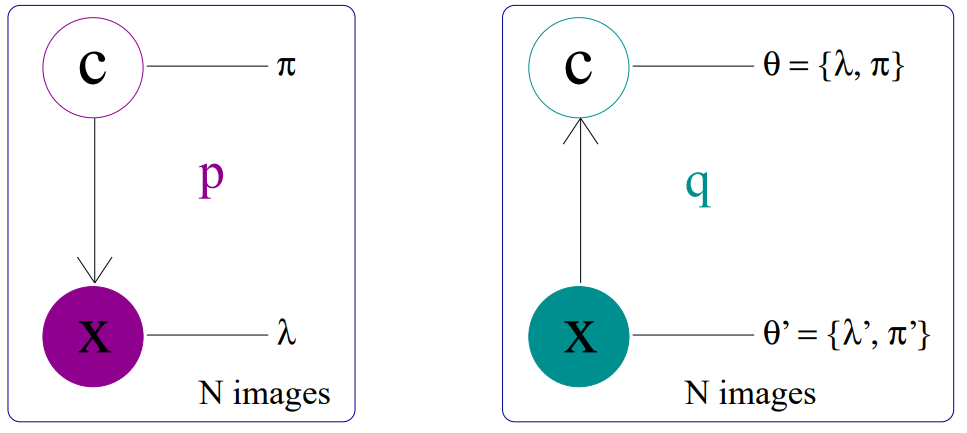
\includegraphics[width=1\textwidth]{pres_img.png}      
\end{column}
\end{columns}
\bigskip
This paper discusses how to use
a Bayesian approach to find automatically the appropriate trade-off between
the generative and discriminative extremes.
\end{frame}
\end{document}